\documentclass[10pt,a4paper]{article}
\usepackage[latin1]{inputenc}
\usepackage{amsmath}
\usepackage{amsfonts}
\usepackage{amssymb}
\usepackage{clrscode}
\usepackage{tikz}
\author{Wendy Moniuk - 996659343}
\title{CSC263 A2}



\tikzset{
 treenode/.style = {align=center, inner sep=0pt, text centered,
    font=\sffamily},
  arn_n/.style = {treenode, circle, black, font=\sffamily\bfseries, draw=black,
    fill=white, text width=1.5em},% arbre rouge noir, noeud noir
  arn_x/.style = {treenode, rectangle, draw=black,
    minimum width=0.5em, minimum height=0.5em}% arbre rouge noir, nil

}

\begin{document}
\maketitle
\begin{enumerate}
\item
\begin{enumerate}

\item
\begin{tikzpicture}[level/.style={sibling distance=60mm/#1}] 
  \node [arn_n][label=$+$] {8}
  		child{ node [label=$-$][arn_n] {4}
  			child{ node [label=$-$][arn_n] {3}
  				child { node [label=$0$] [arn_n] {1} }
  				child { node [arn_x] {} }
  			}
  			child{ node [label=$0$] [arn_n] {5}}
  		}
  		child{ node [label=$-$][arn_n] {15}
  			child{node [label=$-$][arn_n]{11}
  				child{node [label=$+$][arn_n]{9}
  					child{node[arn_x]{}}
  					child{node [label=$0$][arn_n]{10}}
  				}
  				child{node [label=$0$][arn_n]{13}}  			
  			}
  			child{node [label=$+$][arn_n]{18}
  				child{node[arn_x]{}}
  				child{node [label=$0$][arn_n]{20}}  		
                        }
                }
	;
\end{tikzpicture}
\item
\begin{tikzpicture}[level/.style={sibling distance=60mm/#1}]
  \node [arn_n] [label=$0$] {11}
  		child{ node  [label=$0$][arn_n] {8}
  			child{ node [label=$0$] [arn_n] {3}
  				child { node[label=$0$] [arn_n] {1} }
  				child { node [label=$0$][arn_n] {5} }
  			}
  			child{ node[label=$+$] [arn_n] {9}
  				child{ node[arn_x]{}}
  				child{ node [label=$0$][arn_n]{10}}
  			}
  		  		}
  		child{ node[label=$+$] [arn_n] {15}
  			child{node [label=$0$][arn_n]{13}}
  			child{node [label=$+$][arn_n]{18}
  				child{node[arn_x]{}}
  				child{node[label=$0$][arn_n]{20}
  				}  		
  		}
  		}
  		;
\end{tikzpicture}
\end{enumerate}
\item
\begin{enumerate}
\item $m_h = m_{h-1} + m_{h-2} - m_{h-5}, h > 1$ with

<<<<<<< HEAD
$m_{-3} = m_{-2} = m_{-1}= 0, m_0 =1, m_1 = 2$
=======
$m_{-5} = m_{-4} = m_{-3} = m_{-2} = m_{-1}= 0, m_0 =1, m_1 = 2$
>>>>>>> a14aaa258ce9dd9df62c2d8b86f8320191211104

I found the sequence to be $1, 2, 3, 5, 8, 12, 18, 27, 40$ starting from the tree of height 0 and increasing by 1. The pattern starts out like the Fibonacci sequence, but there is a correction factor needed for 
$h \geq 5$ that follows the Fibonacci sequence as well. 

\item
$m_0 = 1 > 1.4^0 - 1 = 0$

$m_1 = 2 > 1.4^1 - 1 = 0.4$

$m_2 = 3 > 1.96 - 1$

$m_3 = 5 > 2.744 - 1$

$m_4 = 8 > 3.8416 - 1$

Assume that it is true for some $m_h$ where 
$h > 4$

Then $m_{h+1} = m_h + m_{h-1} - m_{h-5} \geq 1.4^h - 1 + 1.4^{h-1} - 1 - 1.4^{h-5} + 1 = 1.4^{h}(1+ 1.4^{-1} - 1.4^{-5}) - 1 > 1.4^h(1+ 0.7 - 0.18) -1 > 1.4^h(1.4) - 1 = 1.4^{h+1} -1$

\end{enumerate}
\item
\begin{enumerate}
<<<<<<< HEAD
\item An AVL tree supports all of these operations, all in $O(\log n)$ time.. 
=======
\item A AVL tree supports all of these operations in the correct run time without modifications. 
>>>>>>> a14aaa258ce9dd9df62c2d8b86f8320191211104
\item 
\begin{codebox}
\Procname{$\proc{IsEmptyRange}(S,a,b)$}
\li \If $S$ is empty
\zi \Then
\li		\Return \const{true}
	\End 
\li \If $S.root.key < a$	
\zi \Then
\li			\Return $\proc{IsEmptyRange}(S.right, a, b)$
	\End
\li \If $S.root.key > b$
\zi	\Then 
\li 		\Return $\proc{IsEmptyRange}(S.left, a, b)$
\End
\li 	\Return \const{false}
	

\end{codebox}

This runs in $O(\log n)$ time because it traverses at most the height of the tree and takes a constant time at each node
\end{enumerate}
\item
\begin{enumerate}
\item The data structure I will use is an AVL tree with the key being the price and each node containing the maximum floor area of its sub-tree. It can contain non-distinct nodes. For each node the right sub-tree contains prices strictly greater than itself and the left sub-tree has prices equal to or less than itself.

The diagram below shows the tree after $(p,s)$ pairs 
$(13, 5), (10, 6), (15, 10)$ have been added.

 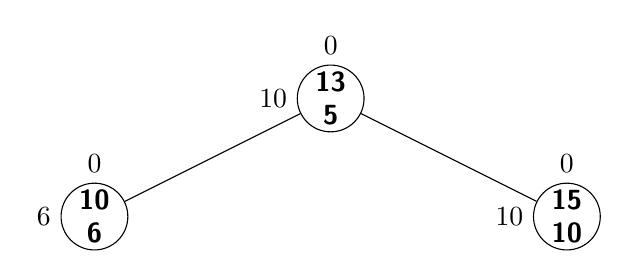
\begin{tikzpicture}[level/.style={sibling distance=60mm/#1}]
    \node [arn_n] [label=$0$] [label=left:$10$] {13 5}
    child { node [arn_n] [label=$0$] [label=left:$6$] {10 6}}
    child { node [arn_n] [label=$0$] [label=left:$10$] {15 10}}
    ;
 \end{tikzpicture}
<<<<<<< HEAD
\item Insert is done at first the usual way for an AVL tree. After a new node is added, or after rebalancing, all the max areas of the ancestors, as well as nodes involved in rotations are updated. The updates would take the same amount of time as the balance factor updates. For delete it is similar, done in the usual way and then max areas are updated.
=======
\item Insert is done at first the usual way for an AVL tree. After a new node is added, or after rebalancing, all the max areas of the ancestors or, nodes involved in rotations, are updated. For delete it is similar, done in the usual way and then max areas are updated.
>>>>>>> a14aaa258ce9dd9df62c2d8b86f8320191211104

For MaxArea, we start at the root and check if p is greater than the root.  An empty tree will return -1. If it is not we call again on the left sub-tree. If it is we keep a variable of the maximum of the max-area of the left sub-tree and the root's area, and call again on to the right sub-tree passing along the current maximum. This is all done in a helper function so we can pass along the current maximum. Once we reach the bottom of the tree we return the maximum over the traversal.

All of these algorithms meet the time requirements. Insert for an AVL tree takes $O(\log n)$ and there will be on the order of log(n) ancestors to update the max-area, where each update takes constant time. Delete for AVL trees also takes 
$O(\log n)$ time, and again there are log(n) ancestors to update. 

MaxArea takes a constant time at each node, 2 comparisons, and it traverses $O(\log n)$ nodes (the height of the tree).
\end{enumerate}
\end{enumerate}
\end{document}
